\section{Dangerzone map based on analysis}
\label{sec:dgrzone}

The thought behind this idea is simple and easy to implement given we have the information needed to do the analysis. The idea is to design a heat map based on some sort of information - in this example we will be using location of radio towers and  the location of forests. The closer to a radio tower, the more heat on the map and as we traverse away from the tower the signal would grow colder. Whenever two signals overlap the heat would rise in that section as illustrated in figure \ref{fig:tempdgr_1}. In our example forests obstruct the signal, therefore creating less signal on the opposing side of the forest, this is illustrated in \ref{fig:tempdgr_2}. With these implications we can build the entire map based on information gathered before the application is launched. 

\begin{figure} [h!]
        \centering
        \begin{subfigure}[b]{0.45\textwidth}
                \frame{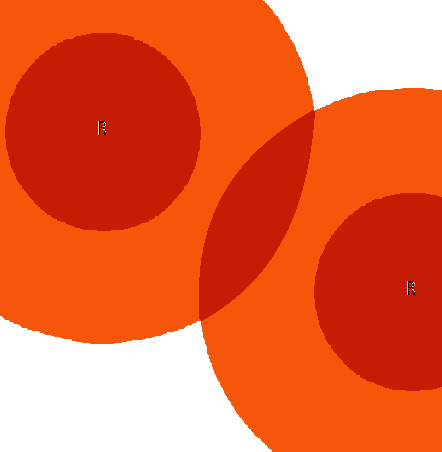
\includegraphics[width=\textwidth]{billeder/tempdgrR}}
                \caption{2 Radiotower signals}
                \label{fig:tempdgr_1}
        \end{subfigure}
        \begin{subfigure}[b]{0.45\textwidth}
                \frame{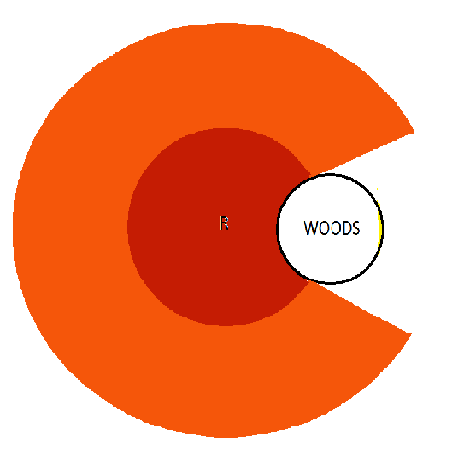
\includegraphics[width=\textwidth]{billeder/tempdgrF}}
                \caption{Signal being obstructed by a forest}
                \label{fig:tempdgr_2}
        \end{subfigure}
        \caption{Illustrations of the idea}\label{fig:temdgr}
\end{figure}

When the heat-map is complete and ready to use, a specific heat point would have to be a trigger point. Solutions that could be implemented when reaching said trigger point is described in \todo{HUSK EN REFERENCE HER - til after triggers afsnit}. Different Internet Service Providers have already created some heat maps based on theoretical calculations, this is very similar to what we would strive to create. An example of said map is the coverage map created by TDC - this is based on users on the tower, distance to the tower and the surroundings. 



\begin{table} [h]
   \begin{center}
   \begin{minipage}{\textwidth}
      \centering
      \begin{tabularx} {\textwidth} { X | X  }
         \hline
		 & \\
         Advantages & Disadvantages \\
		& \\\hline
		& \\
         \tabitem No data besides the map needs to be saved & \tabitem It assumes there's no unexpected interference\\
         \tabitem The map is built before application launch & \tabitem Requires a lot of information beforehand \\
                & \tabitem Requires updates to the map every time new information is out \\
		& \\\hline
      \end{tabularx}
      \caption{this is a dummy}
      \label{tab:dgrzone_adv}
   \end{minipage}
   \end{center}
\end{table}
